\chapter{Экспериментальные результаты}

Предложенная в работе модификация базового алгоритма тестировалась на двух вариантах входных данных: графе рек (\ref{pic:rr}) и 
изолиниях высот (\ref{pic:si}).
\begin{figure}[h]
  \centerline {
    \mbox{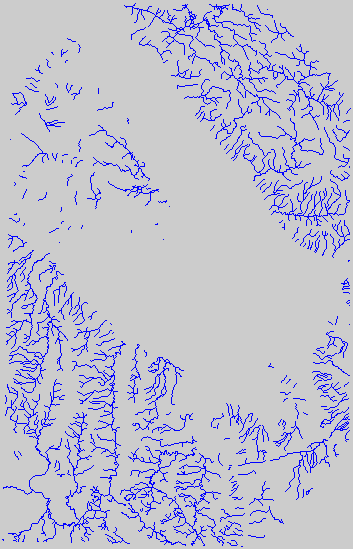
\includegraphics[height=6cm]{rr.png}}
    \mbox{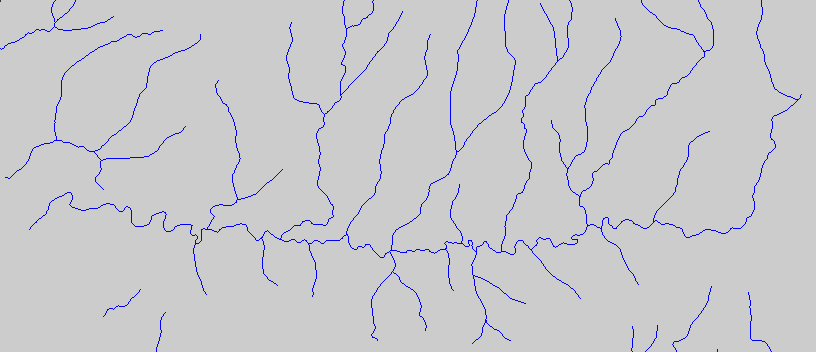
\includegraphics[height=6cm]{rr-small.png}}
  }
  \caption{Рыбинск, реки. $|V_G| = 44482$, $|E_G| = 44274$}
  \label{pic:rr}
\end{figure}
\begin{figure}[h]
  \centerline {
    \mbox{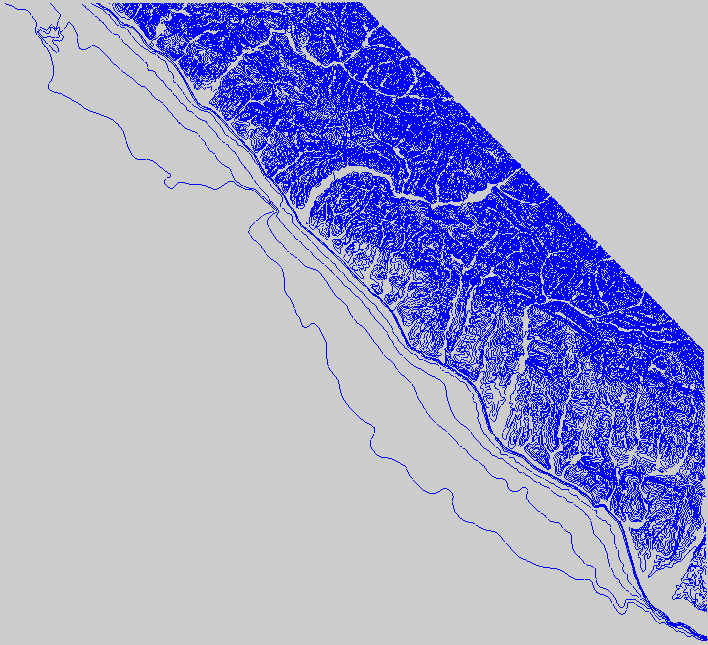
\includegraphics[height=6cm]{si.png}}
    \mbox{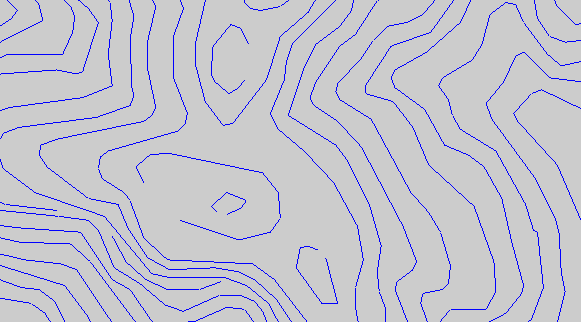
\includegraphics[height=6cm]{si-small.png}}
  }
  \caption{Сочи, изолинии высот. $|V_G| = 81099$, $|E_G| = 79339$}
  \label{pic:si}
\end{figure}

Важно отметить, что предложенная модификация не уменьшает устойчивость ЦВЗ к атакам. Как уже говорилось (\ref{sec:explanation}), 
можно считать, что единственный вид атак, которым подвергается подписанная карта --- аддитивный случайный шум.
\begin{figure} [p]
    \centerline {
        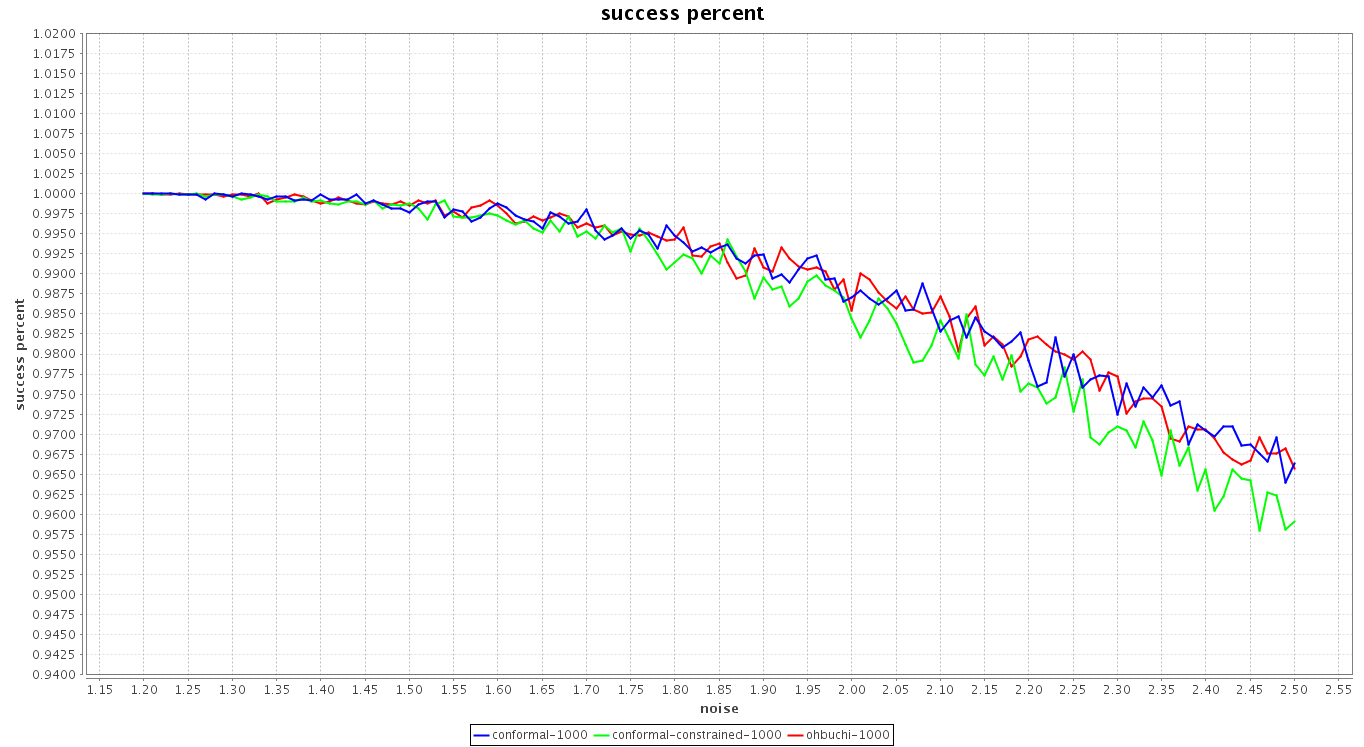
\includegraphics[height=10.5cm]{rr-graphic.png}
    }
    \caption{Устойчивость к шуму, граф рек, шаг амплитуды шума 0.01}
    \label{pic:rr-graphic}
\end{figure}
\begin{figure} [p]
    \centerline {
        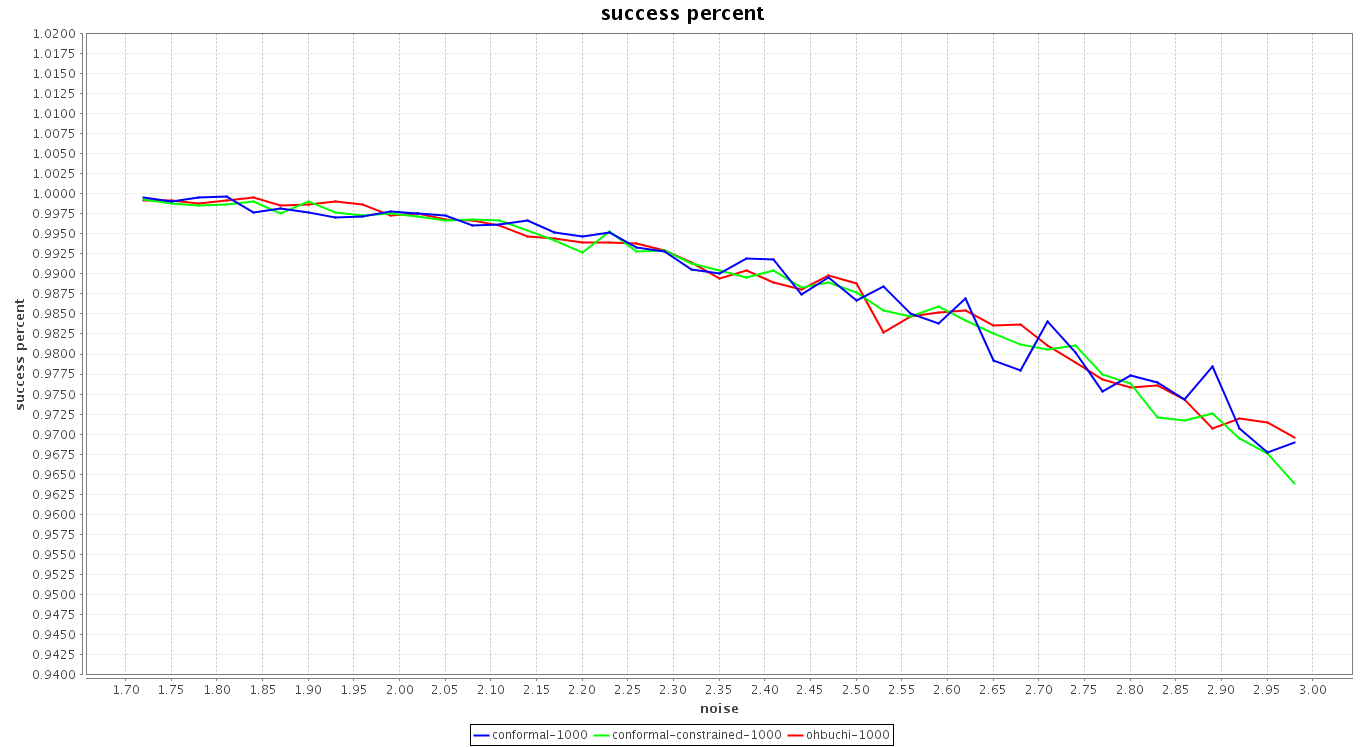
\includegraphics[height=10.5cm]{si-graphic.png}
    }
    \caption{Устойчивость к шуму, изолинии, шаг амплитуды шума 0.03}
    \label{pic:si-graphic}
\end{figure}
На графиках (\ref{pic:rr-graphic}, \ref{pic:si-graphic}), приведена зависимость процента правильно извлеченных битов сообщения от амплитуды 
белого гауссовского шума, с которым была атакована подписанная карта. Красным цветом обозначен результат, показываемый базовым алгоритмом, 
синим --- модификацией базового алгоритма, минимизирующей конформную энергию, зеленым --- модификацией базового алгоритма, 
минимизирующей конформную энергию и использующей триангуляцию с ограничениями.

В обоих случая коэффициет $\alpha = 0.2$, длина внедряемого сообщения~---~119 бит,
максимальное число вершин в областях, на которые делится карта --- 1000, число испытаний, проводимых для каждого значения амплитуды шума --- 50.

Из графиков видно, что минимизация конформной энергии не уменьшает устойчивости ЦВЗ к атакам, использование триангуляции с ограничениями может немного
уменьшить, что, по всей видимости, связано с плохой обусловленностью задачи вычисления собственных векторов взвешенного лапласиана, 
вызываемой почти вырожденными треугольниками.

\begin{figure}[h]
    \centerline {
        \mbox{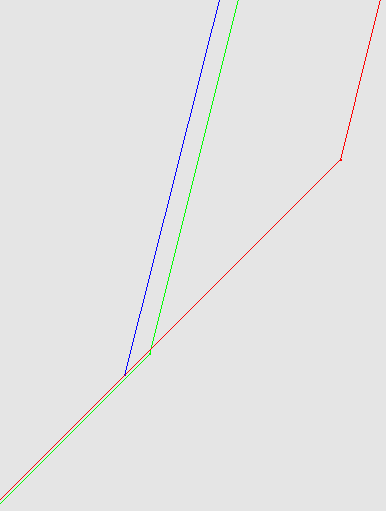
\includegraphics[height=6cm]{angle-diff-small.png}}
        \mbox{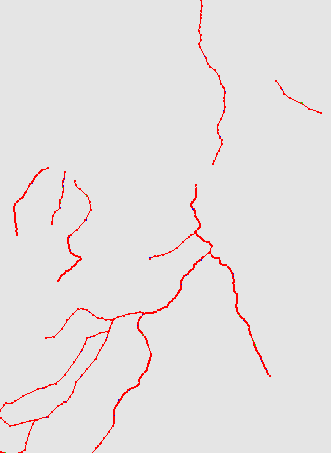
\includegraphics[height=6cm]{angle-diff-large.png}}
    }
    \caption{Карта до и после внедрения ЦВЗ. Слева --- крупный масштаб, справа -- мелкий}
    \label{pic:angle-diff}
\end{figure}

На рис. \ref{pic:angle-diff} зеленым цветом изображена исходная карта, красным цветом --- карта подписанная базовым алгоритмом, 
синим --- карта подписанная модификацией базового алгоритма, минимизирующей конформную энергию. Видно, 
что минимизация предложенного критерия степени искажения исходных данных действительно позволяет уменьшить искажение карты. 

\begin{figure}
    \centerline {
        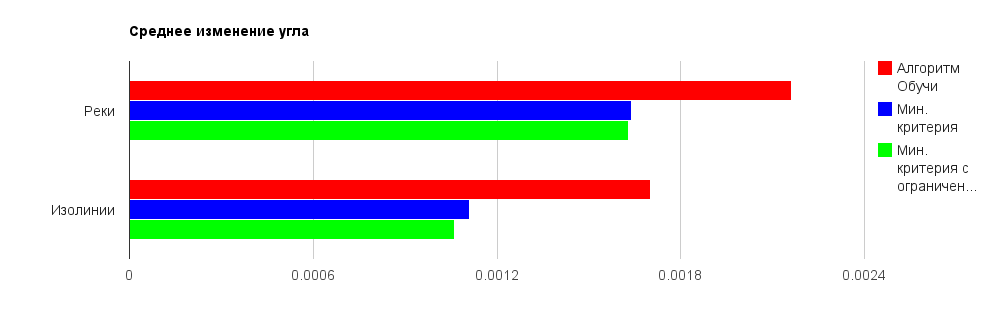
\includegraphics[height=6cm]{histogram.png}
    }
    \caption{Среднее по карте изменение угла}
    \label{pic:histogram}
\end{figure}

Цвета на диаграмме \ref{pic:histogram} соответсвтвуют тем же алгоритмам, что и на графиках (\ref{pic:rr-graphic}, \ref{pic:si-graphic}). 
По диаграмме видно, что предложенная модификация базового алгоритма действительно позволяет минимизировать предложенный критерий стпепени искажения 
исходных данных.

\section{Выводы к главе}
В данной главе было показано, что:
\begin{itemize}
    \item предложенная в работе модификация базового алгоритма не уменьшает устойчивость к атакам;
    \item предложенный в работе критерий степени искажения исходных данных действительно позволяет уменьшить искаженяи карты;
    \item предложенная модификация базового алгоритма позволяет минимизировать предложенный критерий степени искажения исходных данных.
\end{itemize}
